%\begin{center}
%\large \bf \runtitulo
%\end{center}
%\vspace{1cm}
\chapter{Práctico Tema 4}

1. AbueloOAbuela $\equiv$ Persona $\sqcap$ $\exists$hijo-de.PadreOMadre\\ 

AbuelaMaterna $\equiv$ Mujer $\sqcap$ AbueloOAbuela\\


PadreOMadreDeMasDeDos $\equiv$ Persona $\sqcap >= $2 (hijo-de.Persona)\\

HermanoOHermana $\equiv \exists$hijo-de$^-$.PadreOMadreDeMasDeDos\\

SinHijos $\equiv$ Persona $\sqcap$ $\neg$ PadreOMadre\\

TioTia $\equiv$ Persona $\sqcap$ HermanoOHermana $\sqcap$  $\exists$hijo-de$^-$.AbueloOAbuela\\

TioSinHijos $\equiv$ TioTia $\sqcap$ SinHijos\\


AbueloOAbuelaDeMasDeDos $\equiv$ PadreOMadreDeMasDeDos $\sqcap$ AbueloOAbuela\\

PadreDelSobrinoDeUnaNuera $\equiv \exists$ hijo-de$^-$.AbueloOAbuelaDeMasDeDos \\

SobrinoDeUnaNuera $\equiv$ Hombre $\sqcap$ $\exists$hijo-de$^-$.(PadreDelSobrinoDeUnaNuera)\\


PadreConAlMenos3HijosDosMujeres $\equiv$ Persona $\sqcap >=$3 (hijo-de.Persona) $\sqcap >=$2 (hijo-de.Mujer) $\sqcap <=$2 (hijo-de.Mujer)\\


2. Teniendo el siguiente programa en Datalog:

\begin{enumerate}
	\item $father(alice, bob).$
	\item $mother(alice, carla).$
	\item $mother(evan, carla).$
	\item $father(carla, david).$

	\item $parent(X, Y) \gets father(X, Y)$
	\item $parent(X, Y) \gets mother(X, Y)$
	\item $ancestor(X, Y) \gets parent(X, Y)$
	\item $ancestor(X,Z) \gets parent(X, Y) \land ancestor(Y, Z)$
\end{enumerate}

Para derivar $parent(evan, david)$ uno debe apoyarse en las reglas 5 y 6 sería necesario que $father(evan, david).$ o $father(evan, david).$ existieran. Como no es el caso, $parent(evan, david)$ no se puede derivar. \\

Para el caso de $ancestro(carla, david)$, si es posible la derivación. A continuación, se presenta el árbol: \\

\begin{center}
	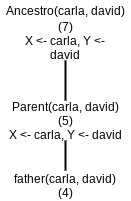
\includegraphics[]{Images/guia4ejercicio2.png}
	\captionof{figure}{Árbol de derivación}
	\label{fig:overview}
\end{center}



3. Debemos agregar la regla: \\

$Q(X, Y) \gets parent(X, Y) \land parent(Z, Y).$\\

Este es el resultado de la consulta Q(X, Y) sería el equivalente a $parent(X, Y)$; en ABCDatalog: \\

$\{Q(alice, bob), Q(alice, carla), Q(carla, david), Q(evan, carla)\}$ \\

4. Debería agregar la regla $Q_{1} \gets parent(X, Y) \land parent(Z, Y).$ para la consulta booleana. \\

5. De esta forma queda el mundo de bloques modelado en Datalog: \\

$estaSobre(b, a).$\\

$tresBloques(a).$
$tresBloques(b).$
$tresBloques(c).$\\

$estaSobreTresBloques(X, Y) \gets tresBloques(X), tresBloques(Y), X \neq Y, estaSobre(X, Y).$ \\

$estaSobreMesa(X) \gets tresBloques(X), tresBloques(Y), tresBloques(Z), X \neq Y,  X \neq Z, Y \neq Z, not estaSobre(X, Y), not estaSobre(X, Z).$\\

$estaApiladoSobre(X, Y) \gets estaApiladoSobreInmediatamente(X, Y).
estaApiladoSobre(X, Y) \gets estaApiladoSobre(X, Z), estaApiladoSobre(Z, Y).$\\

$estaDebajo(X, Y) \gets estaApiladoSobre(Y, X).$\\

$estaApiladoSobreInmediatamente(X, Y) \gets estaSobreTresBloques(X, Y).$\\

$estaDebajoInmediatamente(X, Y) \gets estaSobreTresBloques(Y, X).$\\

$puedeDesapilar(X) \gets tresBloques(X), tresBloques(Y), tresBloques(Z), X \neq Y,  X \neq Z, Y \neq Z, not estaSobreMesa(X), not estaSobre(Y, X), not estaSobre(Z, X).$\\

6. Esquema fuente: relaciones transacción, usuario, transacción\_cuenta, transacción\_usuario.  \\
Esquema destino: relaciones préstamo, usuario.  \\

En el esquema fuente la transacción está compuesta por un id, un id de usuario, un importe y una fecha. También posee un valor que le permite distinguir entre los distintos tipos de transacciones, entre ellas los préstamos. La relación transacción\_cuenta, agrupa a una transacción con la cuenta que fue utilizada en su proceso, transacción\_usuario hace lo mismo con los usuarios. El préstamo por su lado tiene los mismos datos que la transacción, descartando el que indica su tipo y además posee un contrato asociado que deberá generarse y que no forma parte del esquema origen. Los usuarios son equivalentes. \\

$\forall\ TID, UID, IMPORTE, FECHA, CUENTA$ 

$(transaccion(TDI, "ES\_PRESTAMO", UID, IMPORTE, FECHA)\ \land$ 

$transaccion\_cuenta(TDI, CUENTA) \longrightarrow$

$\exists\ CONTRATO (prestamo(TID, UID, FECHA, IMPORTE, CUENTA, CONTRATO)))$\\

$\forall\ UID, NOM\ (usuario(UID, NOM)\ \longrightarrow usuario(UID, NOM))$ \\

Para el ejemplo, presento el siguiente: \\

\begin{table}[h]
	\begin{tabular}{c|c|c|c|c|c}
		TDI  & UID & IMPORTE & FECHA & CUENTA & TIPO \\ \hline
		1 & 1 & 10,2 & 12/10/1990 &  cuenta1 & $"ES\_PRESTAMO"$ \\
		2 & 2 & 1232,12 & 25/09/2012 & cuenta2 & $"ES\_PAGO"$ \\
	\end{tabular}
\end{table}

\begin{table}[h]
	\begin{tabular}{l|l}
		TDI  & CUENTA \\ \hline
		1 & cuenta1 \\
		2 & cuenta2 \\
	\end{tabular}
\end{table}

\begin{table}[h]
	\begin{tabular}{l|l}
		UID & NOM\\ \hline
		 1 & Karen Sanchez \\
		 2 & Karen Carles  \\
	\end{tabular}
\end{table}

Y el destino queda así: \\

\begin{table}[h]
	\begin{tabular}{c|c|c|c|c|c}
		TDI  & UID & IMPORTE & FECHA & CUENTA & CONTRATO\\ \hline
		1 & 1 & 10,2 & 12/10/1990 &  cuenta1 & contrato1 \\
	\end{tabular}
\end{table}

\begin{table}[h]
	\begin{tabular}{l|l}
		UID  & NOM\\ \hline
		1 & Karen Sanchez \\
		2 & Karen Carles  \\
	\end{tabular}
\end{table}


\bigskip